\documentclass[1p]{elsarticle_modified}
%\bibliographystyle{elsarticle-num}

%\usepackage[colorlinks]{hyperref}
%\usepackage{abbrmath_seonhwa} %\Abb, \Ascr, \Acal ,\Abf, \Afrak
\usepackage{amsfonts}
\usepackage{amssymb}
\usepackage{amsmath}
\usepackage{amsthm}
\usepackage{scalefnt}
\usepackage{amsbsy}
\usepackage{kotex}
\usepackage{caption}
\usepackage{subfig}
\usepackage{color}
\usepackage{graphicx}
\usepackage{xcolor} %% white, black, red, green, blue, cyan, magenta, yellow
\usepackage{float}
\usepackage{setspace}
\usepackage{hyperref}

\usepackage{tikz}
\usetikzlibrary{arrows}

\usepackage{multirow}
\usepackage{array} % fixed length table
\usepackage{hhline}

%%%%%%%%%%%%%%%%%%%%%
\makeatletter
\renewcommand*\env@matrix[1][\arraystretch]{%
	\edef\arraystretch{#1}%
	\hskip -\arraycolsep
	\let\@ifnextchar\new@ifnextchar
	\array{*\c@MaxMatrixCols c}}
\makeatother %https://tex.stackexchange.com/questions/14071/how-can-i-increase-the-line-spacing-in-a-matrix
%%%%%%%%%%%%%%%

\usepackage[normalem]{ulem}

\newcommand{\msout}[1]{\ifmmode\text{\sout{\ensuremath{#1}}}\else\sout{#1}\fi}
%SOURCE: \msout is \stkout macro in https://tex.stackexchange.com/questions/20609/strikeout-in-math-mode

\newcommand{\cancel}[1]{
	\ifmmode
	{\color{red}\msout{#1}}
	\else
	{\color{red}\sout{#1}}
	\fi
}

\newcommand{\add}[1]{
	{\color{blue}\uwave{#1}}
}

\newcommand{\replace}[2]{
	\ifmmode
	{\color{red}\msout{#1}}{\color{blue}\uwave{#2}}
	\else
	{\color{red}\sout{#1}}{\color{blue}\uwave{#2}}
	\fi
}

\newcommand{\Sol}{\mathcal{S}} %segment
\newcommand{\D}{D} %diagram
\newcommand{\A}{\mathcal{A}} %arc


%%%%%%%%%%%%%%%%%%%%%%%%%%%%%5 test

\def\sl{\operatorname{\textup{SL}}(2,\Cbb)}
\def\psl{\operatorname{\textup{PSL}}(2,\Cbb)}
\def\quan{\mkern 1mu \triangleright \mkern 1mu}

\theoremstyle{definition}
\newtheorem{thm}{Theorem}[section]
\newtheorem{prop}[thm]{Proposition}
\newtheorem{lem}[thm]{Lemma}
\newtheorem{ques}[thm]{Question}
\newtheorem{cor}[thm]{Corollary}
\newtheorem{defn}[thm]{Definition}
\newtheorem{exam}[thm]{Example}
\newtheorem{rmk}[thm]{Remark}
\newtheorem{alg}[thm]{Algorithm}

\newcommand{\I}{\sqrt{-1}}
\begin{document}

%\begin{frontmatter}
%
%\title{Boundary parabolic representations of knots up to 8 crossings}
%
%%% Group authors per affiliation:
%\author{Yunhi Cho} 
%\address{Department of Mathematics, University of Seoul, Seoul, Korea}
%\ead{yhcho@uos.ac.kr}
%
%
%\author{Seonhwa Kim} %\fnref{s_kim}}
%\address{Center for Geometry and Physics, Institute for Basic Science, Pohang, 37673, Korea}
%\ead{ryeona17@ibs.re.kr}
%
%\author{Hyuk Kim}
%\address{Department of Mathematical Sciences, Seoul National University, Seoul 08826, Korea}
%\ead{hyukkim@snu.ac.kr}
%
%\author{Seokbeom Yoon}
%\address{Department of Mathematical Sciences, Seoul National University, Seoul, 08826,  Korea}
%\ead{sbyoon15@snu.ac.kr}
%
%\begin{abstract}
%We find all boundary parabolic representation of knots up to 8 crossings.
%
%\end{abstract}
%\begin{keyword}
%    \MSC[2010] 57M25 
%\end{keyword}
%
%\end{frontmatter}

%\linenumbers
%\tableofcontents
%
\newcommand\colored[1]{\textcolor{white}{\rule[-0.35ex]{0.8em}{1.4ex}}\kern-0.8em\color{red} #1}%
%\newcommand\colored[1]{\textcolor{white}{ #1}\kern-2.17ex	\textcolor{white}{ #1}\kern-1.81ex	\textcolor{white}{ #1}\kern-2.15ex\color{red}#1	}

{\Large $\underline{11a_{57}~(K11a_{57})}$}

\setlength{\tabcolsep}{10pt}
\renewcommand{\arraystretch}{1.6}
\vspace{1cm}\begin{tabular}{m{100pt}>{\centering\arraybackslash}m{274pt}}
\multirow{5}{120pt}{
	\centering
	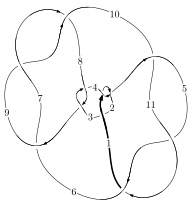
\includegraphics[width=112pt]{../../../GIT/diagram.site/Diagrams/png/306_11a_57.png}\\
\ \ \ A knot diagram\footnotemark}&
\allowdisplaybreaks
\textbf{Linearized knot diagam} \\
\cline{2-2}
 &
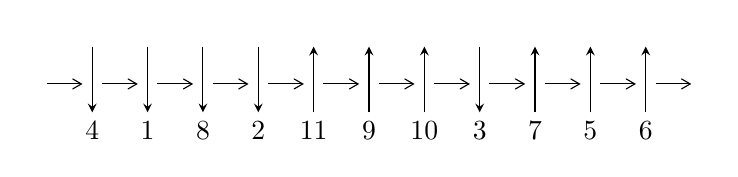
\begin{tikzpicture}[x=20pt, y=17pt]
	% nodes
	\node (C0) at (0, 0) {};
	\node (C1) at (1, 0) {};
	\node (C1U) at (1, +1) {};
	\node (C1D) at (1, -1) {4};

	\node (C2) at (2, 0) {};
	\node (C2U) at (2, +1) {};
	\node (C2D) at (2, -1) {1};

	\node (C3) at (3, 0) {};
	\node (C3U) at (3, +1) {};
	\node (C3D) at (3, -1) {8};

	\node (C4) at (4, 0) {};
	\node (C4U) at (4, +1) {};
	\node (C4D) at (4, -1) {2};

	\node (C5) at (5, 0) {};
	\node (C5U) at (5, +1) {};
	\node (C5D) at (5, -1) {11};

	\node (C6) at (6, 0) {};
	\node (C6U) at (6, +1) {};
	\node (C6D) at (6, -1) {9};

	\node (C7) at (7, 0) {};
	\node (C7U) at (7, +1) {};
	\node (C7D) at (7, -1) {10};

	\node (C8) at (8, 0) {};
	\node (C8U) at (8, +1) {};
	\node (C8D) at (8, -1) {3};

	\node (C9) at (9, 0) {};
	\node (C9U) at (9, +1) {};
	\node (C9D) at (9, -1) {7};

	\node (C10) at (10, 0) {};
	\node (C10U) at (10, +1) {};
	\node (C10D) at (10, -1) {5};

	\node (C11) at (11, 0) {};
	\node (C11U) at (11, +1) {};
	\node (C11D) at (11, -1) {6};
	\node (C12) at (12, 0) {};

	% arrows
	\draw[->,>={angle 60}]
	(C0) edge (C1) (C1) edge (C2) (C2) edge (C3) (C3) edge (C4) (C4) edge (C5) (C5) edge (C6) (C6) edge (C7) (C7) edge (C8) (C8) edge (C9) (C9) edge (C10) (C10) edge (C11) (C11) edge (C12) ;	\draw[->,>=stealth]
	(C1U) edge (C1D) (C2U) edge (C2D) (C3U) edge (C3D) (C4U) edge (C4D) (C5D) edge (C5U) (C6D) edge (C6U) (C7D) edge (C7U) (C8U) edge (C8D) (C9D) edge (C9U) (C10D) edge (C10U) (C11D) edge (C11U) ;
	\end{tikzpicture} \\
\hhline{~~} \\& 
\textbf{Solving Sequence} \\ \cline{2-2} 
 &
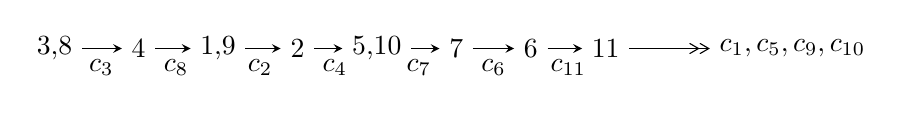
\begin{tikzpicture}[x=27pt, y=7pt]
	% node
	\node (A0) at (-1/8, 0) {3,8};
	\node (A1) at (1, 0) {4};
	\node (A2) at (33/16, 0) {1,9};
	\node (A3) at (25/8, 0) {2};
	\node (A4) at (67/16, 0) {5,10};
	\node (A5) at (21/4, 0) {7};
	\node (A6) at (25/4, 0) {6};
	\node (A7) at (29/4, 0) {11};
	\node (C1) at (1/2, -1) {$c_{3}$};
	\node (C2) at (3/2, -1) {$c_{8}$};
	\node (C3) at (21/8, -1) {$c_{2}$};
	\node (C4) at (29/8, -1) {$c_{4}$};
	\node (C5) at (19/4, -1) {$c_{7}$};
	\node (C6) at (23/4, -1) {$c_{6}$};
	\node (C7) at (27/4, -1) {$c_{11}$};
	\node (A8) at (39/4, 0) {$c_{1},c_{5},c_{9},c_{10}$};

	% edge
	\draw[->,>=stealth]	
	(A0) edge (A1) (A1) edge (A2) (A2) edge (A3) (A3) edge (A4) (A4) edge (A5) (A5) edge (A6) (A6) edge (A7) ;
	\draw[->>,>={angle 60}]	
	(A7) edge (A8);
\end{tikzpicture} \\ 

\end{tabular} \\

\footnotetext{
The image of knot diagram is generated by the software ``\textbf{Draw programme}" developed by Andrew Bartholomew(\url{http://www.layer8.co.uk/maths/draw/index.htm\#Running-draw}), where we modified some parts for our purpose(\url{https://github.com/CATsTAILs/LinksPainter}).
}\phantom \\ \newline 
\centering \textbf{Ideals for irreducible components\footnotemark of $X_{\text{par}}$} 
 
\begin{align*}
I^u_{1}&=\langle 
-68209745 u^{16}+103218620 u^{15}+\cdots+6895752724 d+558230980,\\
\phantom{I^u_{1}}&\phantom{= \langle  }-117728333 u^{16}+37441650 u^{15}+\cdots+13791505448 c-2779791176,\\
\phantom{I^u_{1}}&\phantom{= \langle  }-70376587 u^{16}+38764471 u^{15}+\cdots+6895752724 b+3895994728,\\
\phantom{I^u_{1}}&\phantom{= \langle  }-327083412 u^{16}+276473252 u^{15}+\cdots+6895752724 a-7902639380,\;u^{17}-2 u^{16}+\cdots-4 u^2+8\rangle \\
I^u_{2}&=\langle 
u^6 c+2 u^5 c+3 u^4 c+2 u^3 c- u^3- c u- u^2+d- u,\\
\phantom{I^u_{2}}&\phantom{= \langle  }- u^6 c- u^5 c-2 u^4 c- u^3 c- u^2 c+2 c^2- c u-2 u^2-2 u-2,\;- u^4- u^3- u^2+b+1,\\
\phantom{I^u_{2}}&\phantom{= \langle  }- u^6-3 u^5-4 u^4-3 u^3- u^2+2 a+u,\;u^7+3 u^6+6 u^5+7 u^4+5 u^3+u^2-2 u-2\rangle \\
I^u_{3}&=\langle 
- u^4+d,\;- u^2+c-1,\;- u^4 a-2 u^2 a+u^3- a u+b- a+u+1,\\
\phantom{I^u_{3}}&\phantom{= \langle  }u^3 a-2 u^2 a- u^3+a^2+2 a u+u^2-2 a- u+1,\;u^5- u^4+2 u^3- u^2+u-1\rangle \\
I^u_{4}&=\langle 
2 u^4 a-2 u^4+4 u^2 a+2 u^3+a u-6 u^2+d+4 a+2 u-4,\;- u^4 a+u^4-2 u^2 a- u^3+3 u^2+c-2 a- u+2,\\
\phantom{I^u_{4}}&\phantom{= \langle  }- u^4 a-2 u^2 a+u^3- a u+b- a+u+1,\;u^3 a-2 u^2 a- u^3+a^2+2 a u+u^2-2 a- u+1,\\
\phantom{I^u_{4}}&\phantom{= \langle  }u^5- u^4+2 u^3- u^2+u-1\rangle \\
I^u_{5}&=\langle 
- u^4+d,\;- u^2+c-1,\;u^4- u^3+u^2+b+1,\;2 u^4- u^3+4 u^2+a+2,\;u^5- u^4+2 u^3- u^2+u-1\rangle \\
\\
I^v_{1}&=\langle 
c,\;d-1,\;b,\;a-1,\;v+1\rangle \\
I^v_{2}&=\langle 
a,\;d,\;c-1,\;b+1,\;v-1\rangle \\
I^v_{3}&=\langle 
a,\;d+1,\;c- a,\;b+1,\;v-1\rangle \\
I^v_{4}&=\langle 
a,\;d a+c-1,\;d v+1,\;c v- a- v,\;b+1\rangle \\
\end{align*}
\raggedright * 8 irreducible components of $\dim_{\mathbb{C}}=0$, with total 59 representations.\\
\raggedright * 1 irreducible components of $\dim_{\mathbb{C}}=1$ \\
\footnotetext{All coefficients of polynomials are rational numbers. But the coefficients are sometimes approximated in decimal forms when there is not enough margin.}
\newpage
\renewcommand{\arraystretch}{1}
\centering \section*{I. $I^u_{1}= \langle -6.82\times10^{7} u^{16}+1.03\times10^{8} u^{15}+\cdots+6.90\times10^{9} d+5.58\times10^{8},\;-1.18\times10^{8} u^{16}+3.74\times10^{7} u^{15}+\cdots+1.38\times10^{10} c-2.78\times10^{9},\;-7.04\times10^{7} u^{16}+3.88\times10^{7} u^{15}+\cdots+6.90\times10^{9} b+3.90\times10^{9},\;-3.27\times10^{8} u^{16}+2.76\times10^{8} u^{15}+\cdots+6.90\times10^{9} a-7.90\times10^{9},\;u^{17}-2 u^{16}+\cdots-4 u^2+8 \rangle$}
\flushleft \textbf{(i) Arc colorings}\\
\begin{tabular}{m{7pt} m{180pt} m{7pt} m{180pt} }
\flushright $a_{3}=$&$\begin{pmatrix}1\\0\end{pmatrix}$ \\
\flushright $a_{8}=$&$\begin{pmatrix}0\\u\end{pmatrix}$ \\
\flushright $a_{4}=$&$\begin{pmatrix}1\\u^2\end{pmatrix}$ \\
\flushright $a_{1}=$&$\begin{pmatrix}0.0474326 u^{16}-0.0400933 u^{15}+\cdots+0.133884 u+1.14602\\0.0102058 u^{16}-0.00562150 u^{15}+\cdots+0.589483 u-0.564985\end{pmatrix}$ \\
\flushright $a_{9}=$&$\begin{pmatrix}- u\\u\end{pmatrix}$ \\
\flushright $a_{2}=$&$\begin{pmatrix}-0.0115535 u^{16}-0.0103886 u^{15}+\cdots-0.835060 u+1.27282\\-0.0135318 u^{16}+0.0739510 u^{15}+\cdots+1.06137 u+0.141156\end{pmatrix}$ \\
\flushright $a_{5}=$&$\begin{pmatrix}0.0576384 u^{16}-0.0457148 u^{15}+\cdots+0.723367 u+0.581031\\-0.0339841 u^{16}+0.0141997 u^{15}+\cdots-1.05059 u+0.00848878\end{pmatrix}$ \\
\flushright $a_{10}=$&$\begin{pmatrix}0.00853629 u^{16}-0.00271483 u^{15}+\cdots-0.843158 u+0.201558\\0.00989156 u^{16}-0.0149684 u^{15}+\cdots+0.971920 u-0.0809529\end{pmatrix}$ \\
\flushright $a_{7}=$&$\begin{pmatrix}-0.0184279 u^{16}+0.0176833 u^{15}+\cdots-0.128762 u-0.120605\\0.00989156 u^{16}-0.0149684 u^{15}+\cdots+0.971920 u-0.0809529\end{pmatrix}$ \\
\flushright $a_{6}=$&$\begin{pmatrix}-0.0196690 u^{16}+0.00798947 u^{15}+\cdots-0.197053 u-0.235467\\0.0111327 u^{16}-0.00527464 u^{15}+\cdots+1.04021 u+0.0339091\end{pmatrix}$ \\
\flushright $a_{11}=$&$\begin{pmatrix}0.0321906 u^{16}-0.0342299 u^{15}+\cdots-0.170381 u+0.791078\\0.00701992 u^{16}+0.00619838 u^{15}+\cdots+0.764986 u-0.330652\end{pmatrix}$\\ \flushright $a_{11}=$&$\begin{pmatrix}0.0321906 u^{16}-0.0342299 u^{15}+\cdots-0.170381 u+0.791078\\0.00701992 u^{16}+0.00619838 u^{15}+\cdots+0.764986 u-0.330652\end{pmatrix}$\\&\end{tabular}
\flushleft \textbf{(ii) Obstruction class $= -1$}\\~\\
\flushleft \textbf{(iii) Cusp Shapes $= \frac{975451789}{3447876362} u^{16}-\frac{210120269}{3447876362} u^{15}+\cdots+\frac{8037027246}{1723938181} u-\frac{2146878348}{1723938181}$}\\~\\
\newpage\renewcommand{\arraystretch}{1}
\flushleft \textbf{(iv) u-Polynomials at the component}\newline \\
\begin{tabular}{m{50pt}|m{274pt}}
Crossings & \hspace{64pt}u-Polynomials at each crossing \\
\hline $$\begin{aligned}c_{1},c_{4}\end{aligned}$$&$\begin{aligned}
&u^{17}-2 u^{16}+\cdots-8 u+4
\end{aligned}$\\
\hline $$\begin{aligned}c_{2}\end{aligned}$$&$\begin{aligned}
&u^{17}+6 u^{16}+\cdots+88 u+16
\end{aligned}$\\
\hline $$\begin{aligned}c_{3},c_{8}\end{aligned}$$&$\begin{aligned}
&u^{17}-2 u^{16}+\cdots-4 u^2+8
\end{aligned}$\\
\hline $$\begin{aligned}c_{5},c_{6},c_{7}\\c_{9},c_{10},c_{11}\end{aligned}$$&$\begin{aligned}
&u^{17}+2 u^{16}+\cdots+3 u+1
\end{aligned}$\\
\hline
\end{tabular}\\~\\
\newpage\renewcommand{\arraystretch}{1}
\flushleft \textbf{(v) Riley Polynomials at the component}\newline \\
\begin{tabular}{m{50pt}|m{274pt}}
Crossings & \hspace{64pt}Riley Polynomials at each crossing \\
\hline $$\begin{aligned}c_{1},c_{4}\end{aligned}$$&$\begin{aligned}
&y^{17}-6 y^{16}+\cdots+88 y-16
\end{aligned}$\\
\hline $$\begin{aligned}c_{2}\end{aligned}$$&$\begin{aligned}
&y^{17}+10 y^{16}+\cdots+288 y-256
\end{aligned}$\\
\hline $$\begin{aligned}c_{3},c_{8}\end{aligned}$$&$\begin{aligned}
&y^{17}+6 y^{16}+\cdots+64 y-64
\end{aligned}$\\
\hline $$\begin{aligned}c_{5},c_{6},c_{7}\\c_{9},c_{10},c_{11}\end{aligned}$$&$\begin{aligned}
&y^{17}-20 y^{16}+\cdots+27 y-1
\end{aligned}$\\
\hline
\end{tabular}\\~\\
\newpage\flushleft \textbf{(vi) Complex Volumes and Cusp Shapes}
$$\begin{array}{c|c|c}  
\text{Solutions to }I^u_{1}& \I (\text{vol} + \sqrt{-1}CS) & \text{Cusp shape}\\
 \hline 
\begin{aligned}
u &= \phantom{-}0.679716 + 0.561358 I \\
a &= \phantom{-}0.469715 + 0.071775 I \\
b &= -1.066150 + 0.686891 I \\
c &= -0.482279 - 0.453082 I \\
d &= \phantom{-}0.255516 + 0.765465 I\end{aligned}
 & -3.14388 + 1.09865 I & -5.52136 - 1.09882 I \\ \hline\begin{aligned}
u &= \phantom{-}0.679716 - 0.561358 I \\
a &= \phantom{-}0.469715 - 0.071775 I \\
b &= -1.066150 - 0.686891 I \\
c &= -0.482279 + 0.453082 I \\
d &= \phantom{-}0.255516 - 0.765465 I\end{aligned}
 & -3.14388 - 1.09865 I & -5.52136 + 1.09882 I \\ \hline\begin{aligned}
u &= \phantom{-}0.555749 + 1.023030 I \\
a &= -0.24717 + 1.86349 I \\
b &= -0.86669 - 1.12847 I \\
c &= -0.493632 - 0.522885 I \\
d &= -0.051009 + 0.779355 I\end{aligned}
 & -1.71782 - 5.90288 I & -0.75718 + 7.23695 I \\ \hline\begin{aligned}
u &= \phantom{-}0.555749 - 1.023030 I \\
a &= -0.24717 - 1.86349 I \\
b &= -0.86669 + 1.12847 I \\
c &= -0.493632 + 0.522885 I \\
d &= -0.051009 - 0.779355 I\end{aligned}
 & -1.71782 + 5.90288 I & -0.75718 - 7.23695 I \\ \hline\begin{aligned}
u &= -1.247530 + 0.318357 I \\
a &= \phantom{-}0.505620 + 0.282992 I \\
b &= \phantom{-}0.454441 + 0.853023 I \\
c &= -1.114330 - 0.162230 I \\
d &= -0.517027 + 0.098116 I\end{aligned}
 & \phantom{-}8.60033 - 1.91429 I & \phantom{-}8.38805 + 0.33236 I \\ \hline\begin{aligned}
u &= -1.247530 - 0.318357 I \\
a &= \phantom{-}0.505620 - 0.282992 I \\
b &= \phantom{-}0.454441 - 0.853023 I \\
c &= -1.114330 + 0.162230 I \\
d &= -0.517027 - 0.098116 I\end{aligned}
 & \phantom{-}8.60033 + 1.91429 I & \phantom{-}8.38805 - 0.33236 I\\
 \hline 
 \end{array}$$\newpage$$\begin{array}{c|c|c}  
\text{Solutions to }I^u_{1}& \I (\text{vol} + \sqrt{-1}CS) & \text{Cusp shape}\\
 \hline 
\begin{aligned}
u &= -0.022849 + 0.695780 I \\
a &= \phantom{-}1.92972 - 1.22120 I \\
b &= -0.342039 + 0.295037 I \\
c &= \phantom{-}0.324109 - 0.810541 I \\
d &= \phantom{-}0.054070 + 0.438524 I\end{aligned}
 & \phantom{-}0.88275 + 1.29794 I & \phantom{-}5.86581 - 6.22804 I \\ \hline\begin{aligned}
u &= -0.022849 - 0.695780 I \\
a &= \phantom{-}1.92972 + 1.22120 I \\
b &= -0.342039 - 0.295037 I \\
c &= \phantom{-}0.324109 + 0.810541 I \\
d &= \phantom{-}0.054070 - 0.438524 I\end{aligned}
 & \phantom{-}0.88275 - 1.29794 I & \phantom{-}5.86581 + 6.22804 I \\ \hline\begin{aligned}
u &= \phantom{-}1.235140 + 0.560024 I \\
a &= \phantom{-}0.436143 + 0.137389 I \\
b &= -0.74733 + 1.42693 I \\
c &= \phantom{-}1.046940 - 0.255771 I \\
d &= \phantom{-}0.525994 + 0.171484 I\end{aligned}
 & \phantom{-}6.85439 + 7.49245 I & \phantom{-}6.04980 - 5.00652 I \\ \hline\begin{aligned}
u &= \phantom{-}1.235140 - 0.560024 I \\
a &= \phantom{-}0.436143 - 0.137389 I \\
b &= -0.74733 - 1.42693 I \\
c &= \phantom{-}1.046940 + 0.255771 I \\
d &= \phantom{-}0.525994 - 0.171484 I\end{aligned}
 & \phantom{-}6.85439 - 7.49245 I & \phantom{-}6.04980 + 5.00652 I \\ \hline\begin{aligned}
u &= -0.66454 + 1.33308 I \\
a &= \phantom{-}0.446199 + 0.683104 I \\
b &= \phantom{-}0.944156 - 0.676727 I \\
c &= \phantom{-}0.252205 + 0.988893 I \\
d &= -0.30957 - 2.53920 I\end{aligned}
 & \phantom{-}11.9481 + 8.6770 I & \phantom{-}9.06927 - 4.38269 I \\ \hline\begin{aligned}
u &= -0.66454 - 1.33308 I \\
a &= \phantom{-}0.446199 - 0.683104 I \\
b &= \phantom{-}0.944156 + 0.676727 I \\
c &= \phantom{-}0.252205 - 0.988893 I \\
d &= -0.30957 + 2.53920 I\end{aligned}
 & \phantom{-}11.9481 - 8.6770 I & \phantom{-}9.06927 + 4.38269 I\\
 \hline 
 \end{array}$$\newpage$$\begin{array}{c|c|c}  
\text{Solutions to }I^u_{1}& \I (\text{vol} + \sqrt{-1}CS) & \text{Cusp shape}\\
 \hline 
\begin{aligned}
u &= \phantom{-}0.79652 + 1.26851 I \\
a &= -0.46664 + 1.36075 I \\
b &= -1.06945 - 1.61168 I \\
c &= -0.297727 + 0.961003 I \\
d &= \phantom{-}0.35861 - 2.47585 I\end{aligned}
 & \phantom{-}9.1924 - 14.7354 I & \phantom{-}6.16899 + 8.15927 I \\ \hline\begin{aligned}
u &= \phantom{-}0.79652 - 1.26851 I \\
a &= -0.46664 - 1.36075 I \\
b &= -1.06945 + 1.61168 I \\
c &= -0.297727 - 0.961003 I \\
d &= \phantom{-}0.35861 + 2.47585 I\end{aligned}
 & \phantom{-}9.1924 + 14.7354 I & \phantom{-}6.16899 - 8.15927 I \\ \hline\begin{aligned}
u &= -0.11728 + 1.54547 I \\
a &= \phantom{-}0.161885 - 1.071490 I \\
b &= \phantom{-}0.08928 + 1.57333 I \\
c &= \phantom{-}0.041573 + 1.021680 I \\
d &= -0.05064 - 2.64219 I\end{aligned}
 & \phantom{-}15.7365 + 3.2760 I & \phantom{-}10.07807 - 2.58290 I \\ \hline\begin{aligned}
u &= -0.11728 - 1.54547 I \\
a &= \phantom{-}0.161885 + 1.071490 I \\
b &= \phantom{-}0.08928 - 1.57333 I \\
c &= \phantom{-}0.041573 - 1.021680 I \\
d &= -0.05064 + 2.64219 I\end{aligned}
 & \phantom{-}15.7365 - 3.2760 I & \phantom{-}10.07807 + 2.58290 I \\ \hline\begin{aligned}
u &= -0.429856\phantom{ +0.000000I} \\
a &= \phantom{-}0.529049\phantom{ +0.000000I} \\
b &= -0.792429\phantom{ +0.000000I} \\
c &= \phantom{-}0.446280\phantom{ +0.000000I} \\
d &= -0.531893\phantom{ +0.000000I}\end{aligned}
 & -1.29941\phantom{ +0.000000I} & -8.68290\phantom{ +0.000000I}\\
 \hline 
 \end{array}$$\newpage\newpage\renewcommand{\arraystretch}{1}
\centering \section*{II. $I^u_{2}= \langle u^6 c+2 u^5 c+\cdots+d- u,\;- u^6 c- u^5 c+\cdots+2 c^2-2,\;- u^4- u^3- u^2+b+1,\;- u^6-3 u^5+\cdots+2 a+u,\;u^7+3 u^6+\cdots-2 u-2 \rangle$}
\flushleft \textbf{(i) Arc colorings}\\
\begin{tabular}{m{7pt} m{180pt} m{7pt} m{180pt} }
\flushright $a_{3}=$&$\begin{pmatrix}1\\0\end{pmatrix}$ \\
\flushright $a_{8}=$&$\begin{pmatrix}0\\u\end{pmatrix}$ \\
\flushright $a_{4}=$&$\begin{pmatrix}1\\u^2\end{pmatrix}$ \\
\flushright $a_{1}=$&$\begin{pmatrix}\frac{1}{2} u^6+\frac{3}{2} u^5+\cdots+\frac{1}{2} u^2-\frac{1}{2} u\\u^4+u^3+u^2-1\end{pmatrix}$ \\
\flushright $a_{9}=$&$\begin{pmatrix}- u\\u\end{pmatrix}$ \\
\flushright $a_{2}=$&$\begin{pmatrix}-\frac{1}{2} u^6-\frac{1}{2} u^5+\cdots+\frac{1}{2} u+1\\- u^5- u^4-2 u^3- u^2+1\end{pmatrix}$ \\
\flushright $a_{5}=$&$\begin{pmatrix}\frac{1}{2} u^6+\frac{3}{2} u^5+\cdots-\frac{1}{2} u-1\\- u^5-2 u^4-2 u^3- u^2+u+1\end{pmatrix}$ \\
\flushright $a_{10}=$&$\begin{pmatrix}c\\- u^6 c-2 u^5 c-3 u^4 c-2 u^3 c+u^3+c u+u^2+u\end{pmatrix}$ \\
\flushright $a_{7}=$&$\begin{pmatrix}u^6 c+2 u^5 c+3 u^4 c+2 u^3 c- u^3- c u- u^2- c- u\\- u^6 c-2 u^5 c-3 u^4 c-2 u^3 c+u^3+c u+u^2+u\end{pmatrix}$ \\
\flushright $a_{6}=$&$\begin{pmatrix}u^6 c+2 u^5 c+3 u^4 c+2 u^3 c+u^2 c- u^3- c u- u^2- c- u\\- u^6 c-2 u^5 c-3 u^4 c-2 u^3 c- u^2 c+u^3+c u+u^2+u\end{pmatrix}$ \\
\flushright $a_{11}=$&$\begin{pmatrix}\frac{1}{2} u^6+\frac{1}{2} u^5+\cdots+\frac{1}{2} u^2-\frac{1}{2} u\\- u^4 c+u^5- u^3 c+2 u^4- u^2 c+3 u^3+2 u^2+u-1\end{pmatrix}$\\ \flushright $a_{11}=$&$\begin{pmatrix}\frac{1}{2} u^6+\frac{1}{2} u^5+\cdots+\frac{1}{2} u^2-\frac{1}{2} u\\- u^4 c+u^5- u^3 c+2 u^4- u^2 c+3 u^3+2 u^2+u-1\end{pmatrix}$\\&\end{tabular}
\flushleft \textbf{(ii) Obstruction class $= -1$}\\~\\
\flushleft \textbf{(iii) Cusp Shapes $= 2 u^6+8 u^5+10 u^4+10 u^3-4 u$}\\~\\
\newpage\renewcommand{\arraystretch}{1}
\flushleft \textbf{(iv) u-Polynomials at the component}\newline \\
\begin{tabular}{m{50pt}|m{274pt}}
Crossings & \hspace{64pt}u-Polynomials at each crossing \\
\hline $$\begin{aligned}c_{1},c_{4}\end{aligned}$$&$\begin{aligned}
&(u^7- u^6- u^5+2 u^4+u^3-2 u^2+u+1)^2
\end{aligned}$\\
\hline $$\begin{aligned}c_{2}\end{aligned}$$&$\begin{aligned}
&(u^7+3 u^6+7 u^5+8 u^4+9 u^3+6 u^2+5 u+1)^2
\end{aligned}$\\
\hline $$\begin{aligned}c_{3},c_{8}\end{aligned}$$&$\begin{aligned}
&(u^7+3 u^6+6 u^5+7 u^4+5 u^3+u^2-2 u-2)^2
\end{aligned}$\\
\hline $$\begin{aligned}c_{5},c_{6},c_{7}\\c_{9},c_{10},c_{11}\end{aligned}$$&$\begin{aligned}
&u^{14}+u^{13}+\cdots-4 u-4
\end{aligned}$\\
\hline
\end{tabular}\\~\\
\newpage\renewcommand{\arraystretch}{1}
\flushleft \textbf{(v) Riley Polynomials at the component}\newline \\
\begin{tabular}{m{50pt}|m{274pt}}
Crossings & \hspace{64pt}Riley Polynomials at each crossing \\
\hline $$\begin{aligned}c_{1},c_{4}\end{aligned}$$&$\begin{aligned}
&(y^7-3 y^6+7 y^5-8 y^4+9 y^3-6 y^2+5 y-1)^2
\end{aligned}$\\
\hline $$\begin{aligned}c_{2}\end{aligned}$$&$\begin{aligned}
&(y^7+5 y^6+19 y^5+36 y^4+49 y^3+38 y^2+13 y-1)^2
\end{aligned}$\\
\hline $$\begin{aligned}c_{3},c_{8}\end{aligned}$$&$\begin{aligned}
&(y^7+3 y^6+4 y^5+y^4- y^3+7 y^2+8 y-4)^2
\end{aligned}$\\
\hline $$\begin{aligned}c_{5},c_{6},c_{7}\\c_{9},c_{10},c_{11}\end{aligned}$$&$\begin{aligned}
&y^{14}-11 y^{13}+\cdots-40 y+16
\end{aligned}$\\
\hline
\end{tabular}\\~\\
\newpage\flushleft \textbf{(vi) Complex Volumes and Cusp Shapes}
$$\begin{array}{c|c|c}  
\text{Solutions to }I^u_{2}& \I (\text{vol} + \sqrt{-1}CS) & \text{Cusp shape}\\
 \hline 
\begin{aligned}
u &= -0.984140 + 0.426152 I \\
a &= \phantom{-}0.472917 - 0.120643 I \\
b &= -0.714380 - 0.998080 I \\
c &= -1.198550 - 0.312556 I \\
d &= -0.438334 + 0.145757 I\end{aligned}
 & \phantom{-}1.19445 - 3.93070 I & \phantom{-}1.74059 + 4.87230 I \\ \hline\begin{aligned}
u &= -0.984140 + 0.426152 I \\
a &= \phantom{-}0.472917 - 0.120643 I \\
b &= -0.714380 - 0.998080 I \\
c &= \phantom{-}0.543084 - 0.485903 I \\
d &= -0.376079 + 1.030380 I\end{aligned}
 & \phantom{-}1.19445 - 3.93070 I & \phantom{-}1.74059 + 4.87230 I \\ \hline\begin{aligned}
u &= -0.984140 - 0.426152 I \\
a &= \phantom{-}0.472917 + 0.120643 I \\
b &= -0.714380 + 0.998080 I \\
c &= -1.198550 + 0.312556 I \\
d &= -0.438334 - 0.145757 I\end{aligned}
 & \phantom{-}1.19445 + 3.93070 I & \phantom{-}1.74059 - 4.87230 I \\ \hline\begin{aligned}
u &= -0.984140 - 0.426152 I \\
a &= \phantom{-}0.472917 + 0.120643 I \\
b &= -0.714380 + 0.998080 I \\
c &= \phantom{-}0.543084 + 0.485903 I \\
d &= -0.376079 - 1.030380 I\end{aligned}
 & \phantom{-}1.19445 + 3.93070 I & \phantom{-}1.74059 - 4.87230 I \\ \hline\begin{aligned}
u &= -0.167785 + 1.218780 I \\
a &= \phantom{-}0.529166 + 1.016880 I \\
b &= \phantom{-}0.242061 - 0.924444 I \\
c &= -0.650809 - 0.592102 I \\
d &= -0.300734 + 0.551723 I\end{aligned}
 & \phantom{-}7.14223 - 0.95540 I & \phantom{-}8.68929 + 2.37083 I \\ \hline\begin{aligned}
u &= -0.167785 + 1.218780 I \\
a &= \phantom{-}0.529166 + 1.016880 I \\
b &= \phantom{-}0.242061 - 0.924444 I \\
c &= \phantom{-}0.093897 + 1.158860 I \\
d &= -0.13529 - 2.82138 I\end{aligned}
 & \phantom{-}7.14223 - 0.95540 I & \phantom{-}8.68929 + 2.37083 I\\
 \hline 
 \end{array}$$\newpage$$\begin{array}{c|c|c}  
\text{Solutions to }I^u_{2}& \I (\text{vol} + \sqrt{-1}CS) & \text{Cusp shape}\\
 \hline 
\begin{aligned}
u &= -0.167785 - 1.218780 I \\
a &= \phantom{-}0.529166 - 1.016880 I \\
b &= \phantom{-}0.242061 + 0.924444 I \\
c &= -0.650809 + 0.592102 I \\
d &= -0.300734 - 0.551723 I\end{aligned}
 & \phantom{-}7.14223 + 0.95540 I & \phantom{-}8.68929 - 2.37083 I \\ \hline\begin{aligned}
u &= -0.167785 - 1.218780 I \\
a &= \phantom{-}0.529166 - 1.016880 I \\
b &= \phantom{-}0.242061 + 0.924444 I \\
c &= \phantom{-}0.093897 - 1.158860 I \\
d &= -0.13529 + 2.82138 I\end{aligned}
 & \phantom{-}7.14223 + 0.95540 I & \phantom{-}8.68929 - 2.37083 I \\ \hline\begin{aligned}
u &= -0.654547 + 1.202470 I \\
a &= -0.33478 - 1.51279 I \\
b &= -0.90125 + 1.43610 I \\
c &= \phantom{-}0.292391 + 1.022450 I \\
d &= -0.38305 - 2.56809 I\end{aligned}
 & \phantom{-}3.65356 + 9.93065 I & \phantom{-}3.53972 - 7.33664 I \\ \hline\begin{aligned}
u &= -0.654547 + 1.202470 I \\
a &= -0.33478 - 1.51279 I \\
b &= -0.90125 + 1.43610 I \\
c &= \phantom{-}0.509792 - 0.511513 I \\
d &= \phantom{-}0.118485 + 0.850766 I\end{aligned}
 & \phantom{-}3.65356 + 9.93065 I & \phantom{-}3.53972 - 7.33664 I \\ \hline\begin{aligned}
u &= -0.654547 - 1.202470 I \\
a &= -0.33478 + 1.51279 I \\
b &= -0.90125 - 1.43610 I \\
c &= \phantom{-}0.292391 - 1.022450 I \\
d &= -0.38305 + 2.56809 I\end{aligned}
 & \phantom{-}3.65356 - 9.93065 I & \phantom{-}3.53972 + 7.33664 I \\ \hline\begin{aligned}
u &= -0.654547 - 1.202470 I \\
a &= -0.33478 + 1.51279 I \\
b &= -0.90125 - 1.43610 I \\
c &= \phantom{-}0.509792 + 0.511513 I \\
d &= \phantom{-}0.118485 - 0.850766 I\end{aligned}
 & \phantom{-}3.65356 - 9.93065 I & \phantom{-}3.53972 + 7.33664 I\\
 \hline 
 \end{array}$$\newpage$$\begin{array}{c|c|c}  
\text{Solutions to }I^u_{2}& \I (\text{vol} + \sqrt{-1}CS) & \text{Cusp shape}\\
 \hline 
\begin{aligned}
u &= \phantom{-}0.612945\phantom{ +0.000000I} \\
a &= \phantom{-}0.665400\phantom{ +0.000000I} \\
b &= -0.252863\phantom{ +0.000000I} \\
c &= -1.05845\phantom{ +0.000000I} \\
d &= \phantom{-}1.74513\phantom{ +0.000000I}\end{aligned}
 & \phantom{-}2.33847\phantom{ +0.000000I} & \phantom{-}2.06080\phantom{ +0.000000I} \\ \hline\begin{aligned}
u &= \phantom{-}0.612945\phantom{ +0.000000I} \\
a &= \phantom{-}0.665400\phantom{ +0.000000I} \\
b &= -0.252863\phantom{ +0.000000I} \\
c &= \phantom{-}1.87884\phantom{ +0.000000I} \\
d &= \phantom{-}0.284876\phantom{ +0.000000I}\end{aligned}
 & \phantom{-}2.33847\phantom{ +0.000000I} & \phantom{-}2.06080\phantom{ +0.000000I}\\
 \hline 
 \end{array}$$\newpage\newpage\renewcommand{\arraystretch}{1}
\centering \section*{III. $I^u_{3}= \langle - u^4+d,\;- u^2+c-1,\;- u^4 a+u^3+\cdots- a+1,\;u^3 a- u^3+\cdots-2 a+1,\;u^5- u^4+2 u^3- u^2+u-1 \rangle$}
\flushleft \textbf{(i) Arc colorings}\\
\begin{tabular}{m{7pt} m{180pt} m{7pt} m{180pt} }
\flushright $a_{3}=$&$\begin{pmatrix}1\\0\end{pmatrix}$ \\
\flushright $a_{8}=$&$\begin{pmatrix}0\\u\end{pmatrix}$ \\
\flushright $a_{4}=$&$\begin{pmatrix}1\\u^2\end{pmatrix}$ \\
\flushright $a_{1}=$&$\begin{pmatrix}a\\u^4 a+2 u^2 a- u^3+a u+a- u-1\end{pmatrix}$ \\
\flushright $a_{9}=$&$\begin{pmatrix}- u\\u\end{pmatrix}$ \\
\flushright $a_{2}=$&$\begin{pmatrix}- u^4 a- u^2 a+u^3- a u+u+1\\u^4 a+u^4+u^2 a-2 u^3+a u+2 u^2-2 u\end{pmatrix}$ \\
\flushright $a_{5}=$&$\begin{pmatrix}u^4 a+2 u^2 a- u^3+a u+2 a- u-1\\- u^4+2 u^3- a u-2 u^2+2 u\end{pmatrix}$ \\
\flushright $a_{10}=$&$\begin{pmatrix}u^2+1\\u^4\end{pmatrix}$ \\
\flushright $a_{7}=$&$\begin{pmatrix}- u^4- u^2-1\\u^4\end{pmatrix}$ \\
\flushright $a_{6}=$&$\begin{pmatrix}-1\\- u^2\end{pmatrix}$ \\
\flushright $a_{11}=$&$\begin{pmatrix}- u^4 a- u^2 a+u^3- a u+u+1\\u^4 a+u^4+u^2 a-2 u^3+a u+2 u^2-2 u\end{pmatrix}$\\ \flushright $a_{11}=$&$\begin{pmatrix}- u^4 a- u^2 a+u^3- a u+u+1\\u^4 a+u^4+u^2 a-2 u^3+a u+2 u^2-2 u\end{pmatrix}$\\&\end{tabular}
\flushleft \textbf{(ii) Obstruction class $= -1$}\\~\\
\flushleft \textbf{(iii) Cusp Shapes $= -4 u^3+4 u^2-4 u+6$}\\~\\
\newpage\renewcommand{\arraystretch}{1}
\flushleft \textbf{(iv) u-Polynomials at the component}\newline \\
\begin{tabular}{m{50pt}|m{274pt}}
Crossings & \hspace{64pt}u-Polynomials at each crossing \\
\hline $$\begin{aligned}c_{1},c_{4},c_{5}\\c_{10},c_{11}\end{aligned}$$&$\begin{aligned}
&u^{10}- u^9-2 u^8+4 u^7-4 u^5+3 u^4+u^3-2 u^2+1
\end{aligned}$\\
\hline $$\begin{aligned}c_{2}\end{aligned}$$&$\begin{aligned}
&u^{10}+5 u^9+\cdots+4 u+1
\end{aligned}$\\
\hline $$\begin{aligned}c_{3},c_{8}\end{aligned}$$&$\begin{aligned}
&(u^5- u^4+2 u^3- u^2+u-1)^2
\end{aligned}$\\
\hline $$\begin{aligned}c_{6},c_{7},c_{9}\end{aligned}$$&$\begin{aligned}
&(u^5+u^4-2 u^3- u^2+u-1)^2
\end{aligned}$\\
\hline
\end{tabular}\\~\\
\newpage\renewcommand{\arraystretch}{1}
\flushleft \textbf{(v) Riley Polynomials at the component}\newline \\
\begin{tabular}{m{50pt}|m{274pt}}
Crossings & \hspace{64pt}Riley Polynomials at each crossing \\
\hline $$\begin{aligned}c_{1},c_{4},c_{5}\\c_{10},c_{11}\end{aligned}$$&$\begin{aligned}
&y^{10}-5 y^9+\cdots-4 y+1
\end{aligned}$\\
\hline $$\begin{aligned}c_{2}\end{aligned}$$&$\begin{aligned}
&y^{10}- y^9-6 y^7+22 y^6+6 y^5+45 y^4+15 y^3+22 y^2+4 y+1
\end{aligned}$\\
\hline $$\begin{aligned}c_{3},c_{8}\end{aligned}$$&$\begin{aligned}
&(y^5+3 y^4+4 y^3+y^2- y-1)^2
\end{aligned}$\\
\hline $$\begin{aligned}c_{6},c_{7},c_{9}\end{aligned}$$&$\begin{aligned}
&(y^5-5 y^4+8 y^3-3 y^2- y-1)^2
\end{aligned}$\\
\hline
\end{tabular}\\~\\
\newpage\flushleft \textbf{(vi) Complex Volumes and Cusp Shapes}
$$\begin{array}{c|c|c}  
\text{Solutions to }I^u_{3}& \I (\text{vol} + \sqrt{-1}CS) & \text{Cusp shape}\\
 \hline 
\begin{aligned}
u &= -0.339110 + 0.822375 I \\
a &= \phantom{-}0.445032 - 0.031192 I \\
b &= -1.50324 - 0.38743 I \\
c &= \phantom{-}0.438694 - 0.557752 I \\
d &= \phantom{-}0.003977 + 0.626138 I\end{aligned}
 & \phantom{-}0.32910 + 1.53058 I & \phantom{-}2.51511 - 4.43065 I \\ \hline\begin{aligned}
u &= -0.339110 + 0.822375 I \\
a &= \phantom{-}0.46155 - 2.45660 I \\
b &= -0.703115 + 0.728284 I \\
c &= \phantom{-}0.438694 - 0.557752 I \\
d &= \phantom{-}0.003977 + 0.626138 I\end{aligned}
 & \phantom{-}0.32910 + 1.53058 I & \phantom{-}2.51511 - 4.43065 I \\ \hline\begin{aligned}
u &= -0.339110 - 0.822375 I \\
a &= \phantom{-}0.445032 + 0.031192 I \\
b &= -1.50324 + 0.38743 I \\
c &= \phantom{-}0.438694 + 0.557752 I \\
d &= \phantom{-}0.003977 - 0.626138 I\end{aligned}
 & \phantom{-}0.32910 - 1.53058 I & \phantom{-}2.51511 + 4.43065 I \\ \hline\begin{aligned}
u &= -0.339110 - 0.822375 I \\
a &= \phantom{-}0.46155 + 2.45660 I \\
b &= -0.703115 - 0.728284 I \\
c &= \phantom{-}0.438694 + 0.557752 I \\
d &= \phantom{-}0.003977 - 0.626138 I\end{aligned}
 & \phantom{-}0.32910 - 1.53058 I & \phantom{-}2.51511 + 4.43065 I \\ \hline\begin{aligned}
u &= \phantom{-}0.766826\phantom{ +0.000000I} \\
a &= \phantom{-}0.595741 + 0.124010 I \\
b &= -0.258559 + 0.407825 I \\
c &= \phantom{-}1.58802\phantom{ +0.000000I} \\
d &= \phantom{-}0.345770\phantom{ +0.000000I}\end{aligned}
 & \phantom{-}2.40108\phantom{ +0.000000I} & \phantom{-}3.48110\phantom{ +0.000000I} \\ \hline\begin{aligned}
u &= \phantom{-}0.766826\phantom{ +0.000000I} \\
a &= \phantom{-}0.595741 - 0.124010 I \\
b &= -0.258559 - 0.407825 I \\
c &= \phantom{-}1.58802\phantom{ +0.000000I} \\
d &= \phantom{-}0.345770\phantom{ +0.000000I}\end{aligned}
 & \phantom{-}2.40108\phantom{ +0.000000I} & \phantom{-}3.48110\phantom{ +0.000000I}\\
 \hline 
 \end{array}$$\newpage$$\begin{array}{c|c|c}  
\text{Solutions to }I^u_{3}& \I (\text{vol} + \sqrt{-1}CS) & \text{Cusp shape}\\
 \hline 
\begin{aligned}
u &= \phantom{-}0.455697 + 1.200150 I \\
a &= \phantom{-}0.542114 - 0.781069 I \\
b &= \phantom{-}0.586363 + 0.691742 I \\
c &= -0.232705 + 1.093810 I \\
d &= \phantom{-}0.32314 - 2.69669 I\end{aligned}
 & \phantom{-}5.87256 - 4.40083 I & \phantom{-}6.74431 + 3.49859 I \\ \hline\begin{aligned}
u &= \phantom{-}0.455697 + 1.200150 I \\
a &= -0.04444 + 1.54938 I \\
b &= -0.62145 - 1.31364 I \\
c &= -0.232705 + 1.093810 I \\
d &= \phantom{-}0.32314 - 2.69669 I\end{aligned}
 & \phantom{-}5.87256 - 4.40083 I & \phantom{-}6.74431 + 3.49859 I \\ \hline\begin{aligned}
u &= \phantom{-}0.455697 - 1.200150 I \\
a &= \phantom{-}0.542114 + 0.781069 I \\
b &= \phantom{-}0.586363 - 0.691742 I \\
c &= -0.232705 - 1.093810 I \\
d &= \phantom{-}0.32314 + 2.69669 I\end{aligned}
 & \phantom{-}5.87256 + 4.40083 I & \phantom{-}6.74431 - 3.49859 I \\ \hline\begin{aligned}
u &= \phantom{-}0.455697 - 1.200150 I \\
a &= -0.04444 - 1.54938 I \\
b &= -0.62145 + 1.31364 I \\
c &= -0.232705 - 1.093810 I \\
d &= \phantom{-}0.32314 + 2.69669 I\end{aligned}
 & \phantom{-}5.87256 + 4.40083 I & \phantom{-}6.74431 - 3.49859 I\\
 \hline 
 \end{array}$$\newpage\newpage\renewcommand{\arraystretch}{1}
\centering \section*{IV. $I^u_{4}= \langle 2 u^4 a-2 u^4+\cdots+4 a-4,\;- u^4 a+u^4+\cdots-2 a+2,\;- u^4 a+u^3+\cdots- a+1,\;u^3 a- u^3+\cdots-2 a+1,\;u^5- u^4+2 u^3- u^2+u-1 \rangle$}
\flushleft \textbf{(i) Arc colorings}\\
\begin{tabular}{m{7pt} m{180pt} m{7pt} m{180pt} }
\flushright $a_{3}=$&$\begin{pmatrix}1\\0\end{pmatrix}$ \\
\flushright $a_{8}=$&$\begin{pmatrix}0\\u\end{pmatrix}$ \\
\flushright $a_{4}=$&$\begin{pmatrix}1\\u^2\end{pmatrix}$ \\
\flushright $a_{1}=$&$\begin{pmatrix}a\\u^4 a+2 u^2 a- u^3+a u+a- u-1\end{pmatrix}$ \\
\flushright $a_{9}=$&$\begin{pmatrix}- u\\u\end{pmatrix}$ \\
\flushright $a_{2}=$&$\begin{pmatrix}- u^4 a- u^2 a+u^3- a u+u+1\\u^4 a+u^4+u^2 a-2 u^3+a u+2 u^2-2 u\end{pmatrix}$ \\
\flushright $a_{5}=$&$\begin{pmatrix}u^4 a+2 u^2 a- u^3+a u+2 a- u-1\\- u^4+2 u^3- a u-2 u^2+2 u\end{pmatrix}$ \\
\flushright $a_{10}=$&$\begin{pmatrix}u^4 a- u^4+2 u^2 a+u^3-3 u^2+2 a+u-2\\-2 u^4 a+2 u^4-4 u^2 a-2 u^3- a u+6 u^2-4 a-2 u+4\end{pmatrix}$ \\
\flushright $a_{7}=$&$\begin{pmatrix}u^4 a- u^4+2 u^2 a+u^3+a u-3 u^2+2 a+u-2\\-2 u^4 a+2 u^4-4 u^2 a-2 u^3- a u+6 u^2-4 a-2 u+4\end{pmatrix}$ \\
\flushright $a_{6}=$&$\begin{pmatrix}2 u^4 a- u^3 a-2 u^4+4 u^2 a+u^3+a u-4 u^2+3 a-2\\-3 u^4 a+u^3 a+3 u^4-6 u^2 a-2 u^3- a u+7 u^2-5 a- u+4\end{pmatrix}$ \\
\flushright $a_{11}=$&$\begin{pmatrix}3 u^4 a-2 u^4+5 u^2 a+u^3+a u-4 u^2+4 a-3\\-3 u^4 a+3 u^4-5 u^2 a-2 u^3- a u+6 u^2-4 a- u+4\end{pmatrix}$\\ \flushright $a_{11}=$&$\begin{pmatrix}3 u^4 a-2 u^4+5 u^2 a+u^3+a u-4 u^2+4 a-3\\-3 u^4 a+3 u^4-5 u^2 a-2 u^3- a u+6 u^2-4 a- u+4\end{pmatrix}$\\&\end{tabular}
\flushleft \textbf{(ii) Obstruction class $= -1$}\\~\\
\flushleft \textbf{(iii) Cusp Shapes $= -4 u^3+4 u^2-4 u+6$}\\~\\
\newpage\renewcommand{\arraystretch}{1}
\flushleft \textbf{(iv) u-Polynomials at the component}\newline \\
\begin{tabular}{m{50pt}|m{274pt}}
Crossings & \hspace{64pt}u-Polynomials at each crossing \\
\hline $$\begin{aligned}c_{1},c_{4},c_{6}\\c_{7},c_{9}\end{aligned}$$&$\begin{aligned}
&u^{10}- u^9-2 u^8+4 u^7-4 u^5+3 u^4+u^3-2 u^2+1
\end{aligned}$\\
\hline $$\begin{aligned}c_{2}\end{aligned}$$&$\begin{aligned}
&u^{10}+5 u^9+\cdots+4 u+1
\end{aligned}$\\
\hline $$\begin{aligned}c_{3},c_{8}\end{aligned}$$&$\begin{aligned}
&(u^5- u^4+2 u^3- u^2+u-1)^2
\end{aligned}$\\
\hline $$\begin{aligned}c_{5},c_{10},c_{11}\end{aligned}$$&$\begin{aligned}
&(u^5+u^4-2 u^3- u^2+u-1)^2
\end{aligned}$\\
\hline
\end{tabular}\\~\\
\newpage\renewcommand{\arraystretch}{1}
\flushleft \textbf{(v) Riley Polynomials at the component}\newline \\
\begin{tabular}{m{50pt}|m{274pt}}
Crossings & \hspace{64pt}Riley Polynomials at each crossing \\
\hline $$\begin{aligned}c_{1},c_{4},c_{6}\\c_{7},c_{9}\end{aligned}$$&$\begin{aligned}
&y^{10}-5 y^9+\cdots-4 y+1
\end{aligned}$\\
\hline $$\begin{aligned}c_{2}\end{aligned}$$&$\begin{aligned}
&y^{10}- y^9-6 y^7+22 y^6+6 y^5+45 y^4+15 y^3+22 y^2+4 y+1
\end{aligned}$\\
\hline $$\begin{aligned}c_{3},c_{8}\end{aligned}$$&$\begin{aligned}
&(y^5+3 y^4+4 y^3+y^2- y-1)^2
\end{aligned}$\\
\hline $$\begin{aligned}c_{5},c_{10},c_{11}\end{aligned}$$&$\begin{aligned}
&(y^5-5 y^4+8 y^3-3 y^2- y-1)^2
\end{aligned}$\\
\hline
\end{tabular}\\~\\
\newpage\flushleft \textbf{(vi) Complex Volumes and Cusp Shapes}
$$\begin{array}{c|c|c}  
\text{Solutions to }I^u_{4}& \I (\text{vol} + \sqrt{-1}CS) & \text{Cusp shape}\\
 \hline 
\begin{aligned}
u &= -0.339110 + 0.822375 I \\
a &= \phantom{-}0.445032 - 0.031192 I \\
b &= -1.50324 - 0.38743 I \\
c &= \phantom{-}0.366828 + 1.351750 I \\
d &= -0.60839 - 3.08007 I\end{aligned}
 & \phantom{-}0.32910 + 1.53058 I & \phantom{-}2.51511 - 4.43065 I \\ \hline\begin{aligned}
u &= -0.339110 + 0.822375 I \\
a &= \phantom{-}0.46155 - 2.45660 I \\
b &= -0.703115 + 0.728284 I \\
c &= -0.805522 - 0.794001 I \\
d &= -0.252685 + 0.375376 I\end{aligned}
 & \phantom{-}0.32910 + 1.53058 I & \phantom{-}2.51511 - 4.43065 I \\ \hline\begin{aligned}
u &= -0.339110 - 0.822375 I \\
a &= \phantom{-}0.445032 + 0.031192 I \\
b &= -1.50324 + 0.38743 I \\
c &= \phantom{-}0.366828 - 1.351750 I \\
d &= -0.60839 + 3.08007 I\end{aligned}
 & \phantom{-}0.32910 - 1.53058 I & \phantom{-}2.51511 + 4.43065 I \\ \hline\begin{aligned}
u &= -0.339110 - 0.822375 I \\
a &= \phantom{-}0.46155 + 2.45660 I \\
b &= -0.703115 - 0.728284 I \\
c &= -0.805522 + 0.794001 I \\
d &= -0.252685 - 0.375376 I\end{aligned}
 & \phantom{-}0.32910 - 1.53058 I & \phantom{-}2.51511 + 4.43065 I \\ \hline\begin{aligned}
u &= \phantom{-}0.766826\phantom{ +0.000000I} \\
a &= \phantom{-}0.595741 + 0.124010 I \\
b &= -0.258559 + 0.407825 I \\
c &= -0.794011 + 0.436741 I \\
d &= \phantom{-}1.13119 - 0.96858 I\end{aligned}
 & \phantom{-}2.40108\phantom{ +0.000000I} & \phantom{-}3.48110\phantom{ +0.000000I} \\ \hline\begin{aligned}
u &= \phantom{-}0.766826\phantom{ +0.000000I} \\
a &= \phantom{-}0.595741 - 0.124010 I \\
b &= -0.258559 - 0.407825 I \\
c &= -0.794011 - 0.436741 I \\
d &= \phantom{-}1.13119 + 0.96858 I\end{aligned}
 & \phantom{-}2.40108\phantom{ +0.000000I} & \phantom{-}3.48110\phantom{ +0.000000I}\\
 \hline 
 \end{array}$$\newpage$$\begin{array}{c|c|c}  
\text{Solutions to }I^u_{4}& \I (\text{vol} + \sqrt{-1}CS) & \text{Cusp shape}\\
 \hline 
\begin{aligned}
u &= \phantom{-}0.455697 + 1.200150 I \\
a &= \phantom{-}0.542114 - 0.781069 I \\
b &= \phantom{-}0.586363 + 0.691742 I \\
c &= -0.518554 - 0.530425 I \\
d &= -0.147334 + 0.766162 I\end{aligned}
 & \phantom{-}5.87256 - 4.40083 I & \phantom{-}6.74431 + 3.49859 I \\ \hline\begin{aligned}
u &= \phantom{-}0.455697 + 1.200150 I \\
a &= -0.04444 + 1.54938 I \\
b &= -0.62145 - 1.31364 I \\
c &= \phantom{-}0.751259 - 0.563387 I \\
d &= \phantom{-}0.377218 + 0.474060 I\end{aligned}
 & \phantom{-}5.87256 - 4.40083 I & \phantom{-}6.74431 + 3.49859 I \\ \hline\begin{aligned}
u &= \phantom{-}0.455697 - 1.200150 I \\
a &= \phantom{-}0.542114 + 0.781069 I \\
b &= \phantom{-}0.586363 - 0.691742 I \\
c &= -0.518554 + 0.530425 I \\
d &= -0.147334 - 0.766162 I\end{aligned}
 & \phantom{-}5.87256 + 4.40083 I & \phantom{-}6.74431 - 3.49859 I \\ \hline\begin{aligned}
u &= \phantom{-}0.455697 - 1.200150 I \\
a &= -0.04444 - 1.54938 I \\
b &= -0.62145 + 1.31364 I \\
c &= \phantom{-}0.751259 + 0.563387 I \\
d &= \phantom{-}0.377218 - 0.474060 I\end{aligned}
 & \phantom{-}5.87256 + 4.40083 I & \phantom{-}6.74431 - 3.49859 I\\
 \hline 
 \end{array}$$\newpage\newpage\renewcommand{\arraystretch}{1}
\centering \section*{V. $I^u_{5}= \langle - u^4+d,\;- u^2+c-1,\;u^4- u^3+u^2+b+1,\;2 u^4- u^3+4 u^2+a+2,\;u^5- u^4+2 u^3- u^2+u-1 \rangle$}
\flushleft \textbf{(i) Arc colorings}\\
\begin{tabular}{m{7pt} m{180pt} m{7pt} m{180pt} }
\flushright $a_{3}=$&$\begin{pmatrix}1\\0\end{pmatrix}$ \\
\flushright $a_{8}=$&$\begin{pmatrix}0\\u\end{pmatrix}$ \\
\flushright $a_{4}=$&$\begin{pmatrix}1\\u^2\end{pmatrix}$ \\
\flushright $a_{1}=$&$\begin{pmatrix}-2 u^4+u^3-4 u^2-2\\- u^4+u^3- u^2-1\end{pmatrix}$ \\
\flushright $a_{9}=$&$\begin{pmatrix}- u\\u\end{pmatrix}$ \\
\flushright $a_{2}=$&$\begin{pmatrix}-2 u^4-4 u^2- u-2\\-2 u^4+2 u^3-2 u^2+u-2\end{pmatrix}$ \\
\flushright $a_{5}=$&$\begin{pmatrix}-3 u^4+2 u^3-5 u^2-3\\u^4-2 u^3-2 u\end{pmatrix}$ \\
\flushright $a_{10}=$&$\begin{pmatrix}u^2+1\\u^4\end{pmatrix}$ \\
\flushright $a_{7}=$&$\begin{pmatrix}- u^4- u^2-1\\u^4\end{pmatrix}$ \\
\flushright $a_{6}=$&$\begin{pmatrix}-1\\- u^2\end{pmatrix}$ \\
\flushright $a_{11}=$&$\begin{pmatrix}-2 u^4-4 u^2- u-2\\-2 u^4+2 u^3-2 u^2+u-2\end{pmatrix}$\\ \flushright $a_{11}=$&$\begin{pmatrix}-2 u^4-4 u^2- u-2\\-2 u^4+2 u^3-2 u^2+u-2\end{pmatrix}$\\&\end{tabular}
\flushleft \textbf{(ii) Obstruction class $= -1$}\\~\\
\flushleft \textbf{(iii) Cusp Shapes $= -4 u^3+4 u^2-4 u+6$}\\~\\
\newpage\renewcommand{\arraystretch}{1}
\flushleft \textbf{(iv) u-Polynomials at the component}\newline \\
\begin{tabular}{m{50pt}|m{274pt}}
Crossings & \hspace{64pt}u-Polynomials at each crossing \\
\hline $$\begin{aligned}c_{1},c_{4},c_{5}\\c_{6},c_{7},c_{9}\\c_{10},c_{11}\end{aligned}$$&$\begin{aligned}
&u^5+u^4-2 u^3- u^2+u-1
\end{aligned}$\\
\hline $$\begin{aligned}c_{2}\end{aligned}$$&$\begin{aligned}
&u^5+5 u^4+8 u^3+3 u^2- u+1
\end{aligned}$\\
\hline $$\begin{aligned}c_{3},c_{8}\end{aligned}$$&$\begin{aligned}
&u^5- u^4+2 u^3- u^2+u-1
\end{aligned}$\\
\hline
\end{tabular}\\~\\
\newpage\renewcommand{\arraystretch}{1}
\flushleft \textbf{(v) Riley Polynomials at the component}\newline \\
\begin{tabular}{m{50pt}|m{274pt}}
Crossings & \hspace{64pt}Riley Polynomials at each crossing \\
\hline $$\begin{aligned}c_{1},c_{4},c_{5}\\c_{6},c_{7},c_{9}\\c_{10},c_{11}\end{aligned}$$&$\begin{aligned}
&y^5-5 y^4+8 y^3-3 y^2- y-1
\end{aligned}$\\
\hline $$\begin{aligned}c_{2}\end{aligned}$$&$\begin{aligned}
&y^5-9 y^4+32 y^3-35 y^2-5 y-1
\end{aligned}$\\
\hline $$\begin{aligned}c_{3},c_{8}\end{aligned}$$&$\begin{aligned}
&y^5+3 y^4+4 y^3+y^2- y-1
\end{aligned}$\\
\hline
\end{tabular}\\~\\
\newpage\flushleft \textbf{(vi) Complex Volumes and Cusp Shapes}
$$\begin{array}{c|c|c}  
\text{Solutions to }I^u_{5}& \I (\text{vol} + \sqrt{-1}CS) & \text{Cusp shape}\\
 \hline 
\begin{aligned}
u &= -0.339110 + 0.822375 I \\
a &= \phantom{-}0.886294 + 0.706265 I \\
b &= \phantom{-}0.206354 - 0.340852 I \\
c &= \phantom{-}0.438694 - 0.557752 I \\
d &= \phantom{-}0.003977 + 0.626138 I\end{aligned}
 & \phantom{-}0.32910 + 1.53058 I & \phantom{-}2.51511 - 4.43065 I \\ \hline\begin{aligned}
u &= -0.339110 - 0.822375 I \\
a &= \phantom{-}0.886294 - 0.706265 I \\
b &= \phantom{-}0.206354 + 0.340852 I \\
c &= \phantom{-}0.438694 + 0.557752 I \\
d &= \phantom{-}0.003977 - 0.626138 I\end{aligned}
 & \phantom{-}0.32910 - 1.53058 I & \phantom{-}2.51511 + 4.43065 I \\ \hline\begin{aligned}
u &= \phantom{-}0.766826\phantom{ +0.000000I} \\
a &= -4.59272\phantom{ +0.000000I} \\
b &= -1.48288\phantom{ +0.000000I} \\
c &= \phantom{-}1.58802\phantom{ +0.000000I} \\
d &= \phantom{-}0.345770\phantom{ +0.000000I}\end{aligned}
 & \phantom{-}2.40108\phantom{ +0.000000I} & \phantom{-}3.48110\phantom{ +0.000000I} \\ \hline\begin{aligned}
u &= \phantom{-}0.455697 + 1.200150 I \\
a &= \phantom{-}0.410064 + 0.037156 I \\
b &= -1.96491 + 0.62190 I \\
c &= -0.232705 + 1.093810 I \\
d &= \phantom{-}0.32314 - 2.69669 I\end{aligned}
 & \phantom{-}5.87256 - 4.40083 I & \phantom{-}6.74431 + 3.49859 I \\ \hline\begin{aligned}
u &= \phantom{-}0.455697 - 1.200150 I \\
a &= \phantom{-}0.410064 - 0.037156 I \\
b &= -1.96491 - 0.62190 I \\
c &= -0.232705 - 1.093810 I \\
d &= \phantom{-}0.32314 + 2.69669 I\end{aligned}
 & \phantom{-}5.87256 + 4.40083 I & \phantom{-}6.74431 - 3.49859 I\\
 \hline 
 \end{array}$$\newpage\newpage\renewcommand{\arraystretch}{1}
\centering \section*{VI. $I^v_{1}= \langle c,\;d-1,\;b,\;a-1,\;v+1 \rangle$}
\flushleft \textbf{(i) Arc colorings}\\
\begin{tabular}{m{7pt} m{180pt} m{7pt} m{180pt} }
\flushright $a_{3}=$&$\begin{pmatrix}1\\0\end{pmatrix}$ \\
\flushright $a_{8}=$&$\begin{pmatrix}-1\\0\end{pmatrix}$ \\
\flushright $a_{4}=$&$\begin{pmatrix}1\\0\end{pmatrix}$ \\
\flushright $a_{1}=$&$\begin{pmatrix}1\\0\end{pmatrix}$ \\
\flushright $a_{9}=$&$\begin{pmatrix}-1\\0\end{pmatrix}$ \\
\flushright $a_{2}=$&$\begin{pmatrix}1\\0\end{pmatrix}$ \\
\flushright $a_{5}=$&$\begin{pmatrix}1\\0\end{pmatrix}$ \\
\flushright $a_{10}=$&$\begin{pmatrix}0\\1\end{pmatrix}$ \\
\flushright $a_{7}=$&$\begin{pmatrix}-1\\-1\end{pmatrix}$ \\
\flushright $a_{6}=$&$\begin{pmatrix}0\\-1\end{pmatrix}$ \\
\flushright $a_{11}=$&$\begin{pmatrix}1\\1\end{pmatrix}$\\ \flushright $a_{11}=$&$\begin{pmatrix}1\\1\end{pmatrix}$\\&\end{tabular}
\flushleft \textbf{(ii) Obstruction class $= 1$}\\~\\
\flushleft \textbf{(iii) Cusp Shapes $= 12$}\\~\\
\newpage\renewcommand{\arraystretch}{1}
\flushleft \textbf{(iv) u-Polynomials at the component}\newline \\
\begin{tabular}{m{50pt}|m{274pt}}
Crossings & \hspace{64pt}u-Polynomials at each crossing \\
\hline $$\begin{aligned}c_{1},c_{2},c_{3}\\c_{4},c_{8}\end{aligned}$$&$\begin{aligned}
&u
\end{aligned}$\\
\hline $$\begin{aligned}c_{5},c_{9}\end{aligned}$$&$\begin{aligned}
&u-1
\end{aligned}$\\
\hline $$\begin{aligned}c_{6},c_{7},c_{10}\\c_{11}\end{aligned}$$&$\begin{aligned}
&u+1
\end{aligned}$\\
\hline
\end{tabular}\\~\\
\newpage\renewcommand{\arraystretch}{1}
\flushleft \textbf{(v) Riley Polynomials at the component}\newline \\
\begin{tabular}{m{50pt}|m{274pt}}
Crossings & \hspace{64pt}Riley Polynomials at each crossing \\
\hline $$\begin{aligned}c_{1},c_{2},c_{3}\\c_{4},c_{8}\end{aligned}$$&$\begin{aligned}
&y
\end{aligned}$\\
\hline $$\begin{aligned}c_{5},c_{6},c_{7}\\c_{9},c_{10},c_{11}\end{aligned}$$&$\begin{aligned}
&y-1
\end{aligned}$\\
\hline
\end{tabular}\\~\\
\newpage\flushleft \textbf{(vi) Complex Volumes and Cusp Shapes}
$$\begin{array}{c|c|c}  
\text{Solutions to }I^v_{1}& \I (\text{vol} + \sqrt{-1}CS) & \text{Cusp shape}\\
 \hline 
\begin{aligned}
v &= -1.00000\phantom{ +0.000000I} \\
a &= \phantom{-}1.00000\phantom{ +0.000000I} \\
b &= \phantom{-0.000000 } 0 \\
c &= \phantom{-0.000000 } 0 \\
d &= \phantom{-}1.00000\phantom{ +0.000000I}\end{aligned}
 & \phantom{-}3.28987\phantom{ +0.000000I} & \phantom{-}12.0000\phantom{ +0.000000I}\\
 \hline 
 \end{array}$$\newpage\newpage\renewcommand{\arraystretch}{1}
\centering \section*{VII. $I^v_{2}= \langle a,\;d,\;c-1,\;b+1,\;v-1 \rangle$}
\flushleft \textbf{(i) Arc colorings}\\
\begin{tabular}{m{7pt} m{180pt} m{7pt} m{180pt} }
\flushright $a_{3}=$&$\begin{pmatrix}1\\0\end{pmatrix}$ \\
\flushright $a_{8}=$&$\begin{pmatrix}1\\0\end{pmatrix}$ \\
\flushright $a_{4}=$&$\begin{pmatrix}1\\0\end{pmatrix}$ \\
\flushright $a_{1}=$&$\begin{pmatrix}0\\-1\end{pmatrix}$ \\
\flushright $a_{9}=$&$\begin{pmatrix}1\\0\end{pmatrix}$ \\
\flushright $a_{2}=$&$\begin{pmatrix}1\\-1\end{pmatrix}$ \\
\flushright $a_{5}=$&$\begin{pmatrix}0\\1\end{pmatrix}$ \\
\flushright $a_{10}=$&$\begin{pmatrix}1\\0\end{pmatrix}$ \\
\flushright $a_{7}=$&$\begin{pmatrix}1\\0\end{pmatrix}$ \\
\flushright $a_{6}=$&$\begin{pmatrix}1\\0\end{pmatrix}$ \\
\flushright $a_{11}=$&$\begin{pmatrix}1\\-1\end{pmatrix}$\\ \flushright $a_{11}=$&$\begin{pmatrix}1\\-1\end{pmatrix}$\\&\end{tabular}
\flushleft \textbf{(ii) Obstruction class $= 1$}\\~\\
\flushleft \textbf{(iii) Cusp Shapes $= 0$}\\~\\
\newpage\renewcommand{\arraystretch}{1}
\flushleft \textbf{(iv) u-Polynomials at the component}\newline \\
\begin{tabular}{m{50pt}|m{274pt}}
Crossings & \hspace{64pt}u-Polynomials at each crossing \\
\hline $$\begin{aligned}c_{1},c_{10},c_{11}\end{aligned}$$&$\begin{aligned}
&u-1
\end{aligned}$\\
\hline $$\begin{aligned}c_{2},c_{4},c_{5}\end{aligned}$$&$\begin{aligned}
&u+1
\end{aligned}$\\
\hline $$\begin{aligned}c_{3},c_{6},c_{7}\\c_{8},c_{9}\end{aligned}$$&$\begin{aligned}
&u
\end{aligned}$\\
\hline
\end{tabular}\\~\\
\newpage\renewcommand{\arraystretch}{1}
\flushleft \textbf{(v) Riley Polynomials at the component}\newline \\
\begin{tabular}{m{50pt}|m{274pt}}
Crossings & \hspace{64pt}Riley Polynomials at each crossing \\
\hline $$\begin{aligned}c_{1},c_{2},c_{4}\\c_{5},c_{10},c_{11}\end{aligned}$$&$\begin{aligned}
&y-1
\end{aligned}$\\
\hline $$\begin{aligned}c_{3},c_{6},c_{7}\\c_{8},c_{9}\end{aligned}$$&$\begin{aligned}
&y
\end{aligned}$\\
\hline
\end{tabular}\\~\\
\newpage\flushleft \textbf{(vi) Complex Volumes and Cusp Shapes}
$$\begin{array}{c|c|c}  
\text{Solutions to }I^v_{2}& \I (\text{vol} + \sqrt{-1}CS) & \text{Cusp shape}\\
 \hline 
\begin{aligned}
v &= \phantom{-}1.00000\phantom{ +0.000000I} \\
a &= \phantom{-0.000000 } 0 \\
b &= -1.00000\phantom{ +0.000000I} \\
c &= \phantom{-}1.00000\phantom{ +0.000000I} \\
d &= \phantom{-0.000000 } 0\end{aligned}
 & \phantom{-0.000000 } 0 & \phantom{-0.000000 } 0\\
 \hline 
 \end{array}$$\newpage\newpage\renewcommand{\arraystretch}{1}
\centering \section*{VIII. $I^v_{3}= \langle a,\;d+1,\;c- a,\;b+1,\;v-1 \rangle$}
\flushleft \textbf{(i) Arc colorings}\\
\begin{tabular}{m{7pt} m{180pt} m{7pt} m{180pt} }
\flushright $a_{3}=$&$\begin{pmatrix}1\\0\end{pmatrix}$ \\
\flushright $a_{8}=$&$\begin{pmatrix}1\\0\end{pmatrix}$ \\
\flushright $a_{4}=$&$\begin{pmatrix}1\\0\end{pmatrix}$ \\
\flushright $a_{1}=$&$\begin{pmatrix}0\\-1\end{pmatrix}$ \\
\flushright $a_{9}=$&$\begin{pmatrix}1\\0\end{pmatrix}$ \\
\flushright $a_{2}=$&$\begin{pmatrix}1\\-1\end{pmatrix}$ \\
\flushright $a_{5}=$&$\begin{pmatrix}0\\1\end{pmatrix}$ \\
\flushright $a_{10}=$&$\begin{pmatrix}0\\-1\end{pmatrix}$ \\
\flushright $a_{7}=$&$\begin{pmatrix}1\\1\end{pmatrix}$ \\
\flushright $a_{6}=$&$\begin{pmatrix}0\\1\end{pmatrix}$ \\
\flushright $a_{11}=$&$\begin{pmatrix}0\\-1\end{pmatrix}$\\ \flushright $a_{11}=$&$\begin{pmatrix}0\\-1\end{pmatrix}$\\&\end{tabular}
\flushleft \textbf{(ii) Obstruction class $= 1$}\\~\\
\flushleft \textbf{(iii) Cusp Shapes $= 0$}\\~\\
\newpage\renewcommand{\arraystretch}{1}
\flushleft \textbf{(iv) u-Polynomials at the component}\newline \\
\begin{tabular}{m{50pt}|m{274pt}}
Crossings & \hspace{64pt}u-Polynomials at each crossing \\
\hline $$\begin{aligned}c_{1},c_{9}\end{aligned}$$&$\begin{aligned}
&u-1
\end{aligned}$\\
\hline $$\begin{aligned}c_{2},c_{4},c_{6}\\c_{7}\end{aligned}$$&$\begin{aligned}
&u+1
\end{aligned}$\\
\hline $$\begin{aligned}c_{3},c_{5},c_{8}\\c_{10},c_{11}\end{aligned}$$&$\begin{aligned}
&u
\end{aligned}$\\
\hline
\end{tabular}\\~\\
\newpage\renewcommand{\arraystretch}{1}
\flushleft \textbf{(v) Riley Polynomials at the component}\newline \\
\begin{tabular}{m{50pt}|m{274pt}}
Crossings & \hspace{64pt}Riley Polynomials at each crossing \\
\hline $$\begin{aligned}c_{1},c_{2},c_{4}\\c_{6},c_{7},c_{9}\end{aligned}$$&$\begin{aligned}
&y-1
\end{aligned}$\\
\hline $$\begin{aligned}c_{3},c_{5},c_{8}\\c_{10},c_{11}\end{aligned}$$&$\begin{aligned}
&y
\end{aligned}$\\
\hline
\end{tabular}\\~\\
\newpage\flushleft \textbf{(vi) Complex Volumes and Cusp Shapes}
$$\begin{array}{c|c|c}  
\text{Solutions to }I^v_{3}& \I (\text{vol} + \sqrt{-1}CS) & \text{Cusp shape}\\
 \hline 
\begin{aligned}
v &= \phantom{-}1.00000\phantom{ +0.000000I} \\
a &= \phantom{-0.000000 } 0 \\
b &= -1.00000\phantom{ +0.000000I} \\
c &= \phantom{-0.000000 } 0 \\
d &= -1.00000\phantom{ +0.000000I}\end{aligned}
 & \phantom{-0.000000 } 0 & \phantom{-0.000000 } 0\\
 \hline 
 \end{array}$$\newpage\newpage\renewcommand{\arraystretch}{1}
\centering \section*{IX. $I^v_{4}= \langle a,\;d a+c-1,\;d v+1,\;c v- a- v,\;b+1 \rangle$}
\flushleft \textbf{(i) Arc colorings}\\
\begin{tabular}{m{7pt} m{180pt} m{7pt} m{180pt} }
\flushright $a_{3}=$&$\begin{pmatrix}1\\0\end{pmatrix}$ \\
\flushright $a_{8}=$&$\begin{pmatrix}v\\0\end{pmatrix}$ \\
\flushright $a_{4}=$&$\begin{pmatrix}1\\0\end{pmatrix}$ \\
\flushright $a_{1}=$&$\begin{pmatrix}0\\-1\end{pmatrix}$ \\
\flushright $a_{9}=$&$\begin{pmatrix}v\\0\end{pmatrix}$ \\
\flushright $a_{2}=$&$\begin{pmatrix}1\\-1\end{pmatrix}$ \\
\flushright $a_{5}=$&$\begin{pmatrix}0\\1\end{pmatrix}$ \\
\flushright $a_{10}=$&$\begin{pmatrix}1\\d\end{pmatrix}$ \\
\flushright $a_{7}=$&$\begin{pmatrix}v-1\\- d\end{pmatrix}$ \\
\flushright $a_{6}=$&$\begin{pmatrix}-1\\- d\end{pmatrix}$ \\
\flushright $a_{11}=$&$\begin{pmatrix}1\\d-1\end{pmatrix}$\\ \flushright $a_{11}=$&$\begin{pmatrix}1\\d-1\end{pmatrix}$\\&\end{tabular}
\flushleft \textbf{(ii) Obstruction class $= -1$}\\~\\
\flushleft \textbf{(iii) Cusp Shapes $= d^2+v^2+4$}\\~\\
\flushleft \textbf{(iv) u-Polynomials at the component} : It cannot be defined for a positive dimension component.\\~\\
\flushleft \textbf{(v) Riley Polynomials at the component} : It cannot be defined for a positive dimension component.\\~\\
\newpage\flushleft \textbf{(iv) Complex Volumes and Cusp Shapes}
$$\begin{array}{c|c|c} 
\text{Solution to }I^v_{4}& \I (\text{vol} + \sqrt{-1}CS) & \text{Cusp shape}\\
 \hline 
\begin{aligned}
v &= \cdots \\
a &= \cdots \\
b &= \cdots \\
c &= \cdots \\
d &= \cdots\end{aligned}
 & \phantom{-}1.64493\phantom{ +0.000000I} & \phantom{-}2.23718 - 0.09992 I\\
 \hline 
 \end{array}
$$
\newpage\renewcommand{\arraystretch}{1}
\centering \section*{ X. u-Polynomials}
\begin{tabular}{m{50pt}|m{274pt}}
Crossings & \hspace{64pt}u-Polynomials at each crossing \\
\hline $$\begin{aligned}c_{1}\end{aligned}$$&$\begin{aligned}
&u(u-1)^2(u^5+u^4-2 u^3- u^2+u-1)\\
&\cdot(u^7- u^6- u^5+2 u^4+u^3-2 u^2+u+1)^2\\
&\cdot(u^{10}- u^9-2 u^8+4 u^7-4 u^5+3 u^4+u^3-2 u^2+1)^2\\
&\cdot(u^{17}-2 u^{16}+\cdots-8 u+4)
\end{aligned}$\\
\hline $$\begin{aligned}c_{2}\end{aligned}$$&$\begin{aligned}
&u(u+1)^2(u^5+5 u^4+8 u^3+3 u^2- u+1)\\
&\cdot(u^7+3 u^6+7 u^5+8 u^4+9 u^3+6 u^2+5 u+1)^2\\
&\cdot((u^{10}+5 u^9+\cdots+4 u+1)^{2})(u^{17}+6 u^{16}+\cdots+88 u+16)
\end{aligned}$\\
\hline $$\begin{aligned}c_{3},c_{8}\end{aligned}$$&$\begin{aligned}
&u^3(u^5- u^4+2 u^3- u^2+u-1)^5\\
&\cdot((u^7+3 u^6+\cdots-2 u-2)^{2})(u^{17}-2 u^{16}+\cdots-4 u^2+8)
\end{aligned}$\\
\hline $$\begin{aligned}c_{4}\end{aligned}$$&$\begin{aligned}
&u(u+1)^2(u^5+u^4-2 u^3- u^2+u-1)\\
&\cdot(u^7- u^6- u^5+2 u^4+u^3-2 u^2+u+1)^2\\
&\cdot(u^{10}- u^9-2 u^8+4 u^7-4 u^5+3 u^4+u^3-2 u^2+1)^2\\
&\cdot(u^{17}-2 u^{16}+\cdots-8 u+4)
\end{aligned}$\\
\hline $$\begin{aligned}c_{5},c_{10},c_{11}\end{aligned}$$&$\begin{aligned}
&u(u-1)(u+1)(u^5+u^4-2 u^3- u^2+u-1)^3\\
&\cdot(u^{10}- u^9-2 u^8+4 u^7-4 u^5+3 u^4+u^3-2 u^2+1)\\
&\cdot(u^{14}+u^{13}+\cdots-4 u-4)(u^{17}+2 u^{16}+\cdots+3 u+1)
\end{aligned}$\\
\hline $$\begin{aligned}c_{6},c_{7}\end{aligned}$$&$\begin{aligned}
&u(u+1)^2(u^5+u^4-2 u^3- u^2+u-1)^3\\
&\cdot(u^{10}- u^9-2 u^8+4 u^7-4 u^5+3 u^4+u^3-2 u^2+1)\\
&\cdot(u^{14}+u^{13}+\cdots-4 u-4)(u^{17}+2 u^{16}+\cdots+3 u+1)
\end{aligned}$\\
\hline $$\begin{aligned}c_{9}\end{aligned}$$&$\begin{aligned}
&u(u-1)^2(u^5+u^4-2 u^3- u^2+u-1)^3\\
&\cdot(u^{10}- u^9-2 u^8+4 u^7-4 u^5+3 u^4+u^3-2 u^2+1)\\
&\cdot(u^{14}+u^{13}+\cdots-4 u-4)(u^{17}+2 u^{16}+\cdots+3 u+1)
\end{aligned}$\\
\hline
\end{tabular}\newpage\renewcommand{\arraystretch}{1}
\centering \section*{ XI. Riley Polynomials}
\begin{tabular}{m{50pt}|m{274pt}}
Crossings & \hspace{64pt}Riley Polynomials at each crossing \\
\hline $$\begin{aligned}c_{1},c_{4}\end{aligned}$$&$\begin{aligned}
&y(y-1)^2(y^5-5 y^4+8 y^3-3 y^2- y-1)\\
&\cdot(y^7-3 y^6+7 y^5-8 y^4+9 y^3-6 y^2+5 y-1)^2\\
&\cdot((y^{10}-5 y^9+\cdots-4 y+1)^{2})(y^{17}-6 y^{16}+\cdots+88 y-16)
\end{aligned}$\\
\hline $$\begin{aligned}c_{2}\end{aligned}$$&$\begin{aligned}
&y(y-1)^2(y^5-9 y^4+32 y^3-35 y^2-5 y-1)\\
&\cdot(y^7+5 y^6+19 y^5+36 y^4+49 y^3+38 y^2+13 y-1)^2\\
&\cdot(y^{10}- y^9-6 y^7+22 y^6+6 y^5+45 y^4+15 y^3+22 y^2+4 y+1)^2\\
&\cdot(y^{17}+10 y^{16}+\cdots+288 y-256)
\end{aligned}$\\
\hline $$\begin{aligned}c_{3},c_{8}\end{aligned}$$&$\begin{aligned}
&y^3(y^5+3 y^4+4 y^3+y^2- y-1)^5\\
&\cdot(y^7+3 y^6+4 y^5+y^4- y^3+7 y^2+8 y-4)^2\\
&\cdot(y^{17}+6 y^{16}+\cdots+64 y-64)
\end{aligned}$\\
\hline $$\begin{aligned}c_{5},c_{6},c_{7}\\c_{9},c_{10},c_{11}\end{aligned}$$&$\begin{aligned}
&y(y-1)^2(y^5-5 y^4+\cdots- y-1)^{3}(y^{10}-5 y^{9}+\cdots-4 y+1)\\
&\cdot(y^{14}-11 y^{13}+\cdots-40 y+16)(y^{17}-20 y^{16}+\cdots+27 y-1)
\end{aligned}$\\
\hline
\end{tabular}
\vskip 2pc
\end{document}